

\section{Accommodation}

\subsection{A\&O Hostel}

\begin{tikzpicture}
  \begin{scope}[on background layer]
    \node[inner sep=0,outer sep=0] (main) {%
      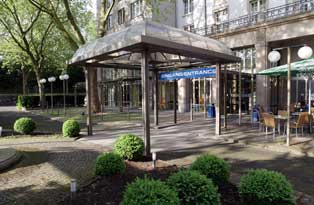
\includegraphics[width=0.25\linewidth]{images/accommodation/auo/bild2.jpg}%
    };
    \node[inner sep=0,outer sep=0,anchor=north west] (img-2) at (main.north east) {%
      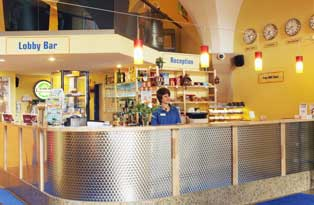
\includegraphics[width=0.25\linewidth]{images/accommodation/auo/bild3.jpg}%
    };
    \node[inner sep=0,outer sep=0,anchor=north west] (img-3) at (img-2.north east) {%
      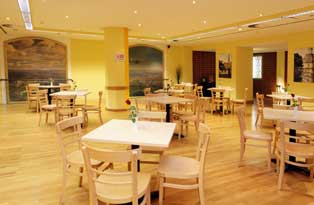
\includegraphics[width=0.25\linewidth]{images/accommodation/auo/bild7.jpg}%
    };
    \node[inner sep=0,outer sep=0,anchor=north west] (img-4) at (img-3.north east) {%
      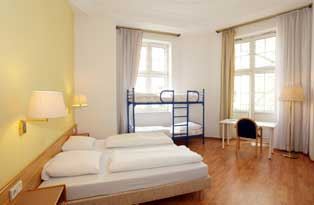
\includegraphics[width=0.25\linewidth]{images/accommodation/auo/bild6.jpg}%
    };
  \end{scope}
  \node[anchor=south west,color=black,xshift=1ex,yshift=1ex] (label) at (main.south west) {\imgtitle{A\&O HOTELS and HOSTELS Holding AG}{A\&O Hostel Karlsruhe}{non-free, permission to use for bid}};
  \begin{scope}[on background layer]
    \node[fit=(label),inner sep=0,outer sep=0,opacity=0.6,fill=white,rounded corners] {};
  \end{scope}
\end{tikzpicture}


\begin{labeling}{\bf Availability}
  \item[\bf Location] Main Station
  \item[\bf Price] single: $\sim\SI{61.30}{/pP}$, 2-3: $\sim\SI{35.30}{/pP}$; 4: $\sim\SI{30.50}{/pP}$
  \item[\bf Breakfast] included, mandatory
  \item[\bf Availability] available
\end{labeling}

This hostel is located right at the main station, which is a little bit off from
the city center. Breakfast is mandatory for group reserverations and the prices
vary quite a lot between the different dates (the estimation is averaged for a
five night stay).

\subsection{Jugendherberge Karlsruhe}

\begin{tikzpicture}
  \begin{scope}[on background layer]
    \node[inner sep=0,outer sep=0] (main) {%
      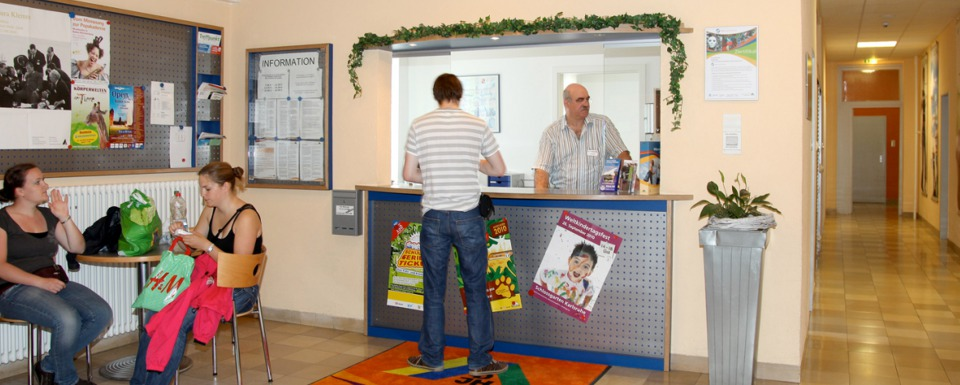
\includegraphics[width=0.5\linewidth]{images/accommodation/jugendherberge/0.jpg}%
    };
    \node[inner sep=0,outer sep=0,anchor=north west] (img-2) at (main.north east) {%
      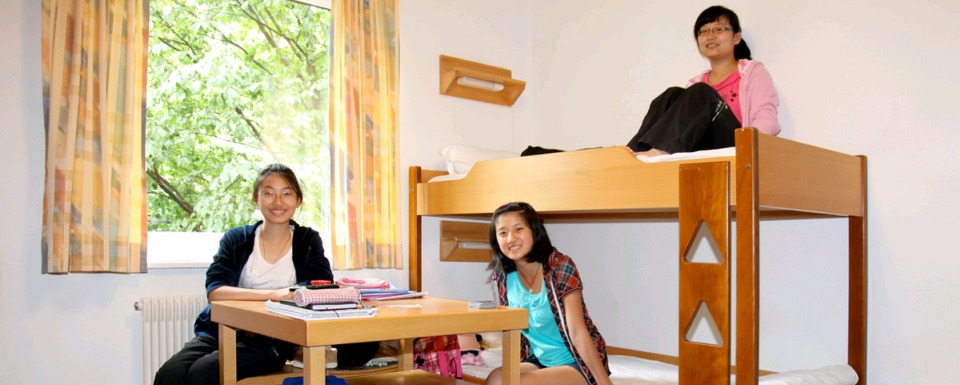
\includegraphics[width=0.5\linewidth]{images/accommodation/jugendherberge/1.jpg}%
    };
  \end{scope}
  \node[anchor=south west,color=black,xshift=1ex,yshift=1ex] (label) at (main.south west) {\imgtitle{Deutsches Jugendherbergswerk Landesverband Baden-Württemberg e.\,V.}{Jugendherberge Karlsruhe}{non-free, permission to use for bid}};
  \begin{scope}[on background layer]
    \node[fit=(label),inner sep=0,outer sep=0,opacity=0.6,fill=white,rounded corners] {};
  \end{scope}
\end{tikzpicture}

\begin{labeling}{\bf Availability}
  \item[\bf Location] North West of City Center
  \item[\bf Price] $\sim\SI{25}{\euro/{pP}}$
  \item[\bf Breakfast] included, mandatory
  \item[\bf Availability] after 21st August
\end{labeling}

The youth hostel is located to the south west of the city center in the middle
of one of the universities, the Hochschule Karlsruhe. The walk to the
next tram station is about \SI{10}{\minute}. While this location would be
pretty affordable, it is heavily used by groups during the summer, and will
not be available to us from the start of Juli till the 21st of August.

Note that it is mandatory to get half-board or a lunch pack for at least some
of the days. The price mentioned here is an estimation that already includes
the extra costs this incurs.

\subsection{Gästehaus Kaiserpassage}

\begin{tikzpicture}
  \begin{scope}[on background layer]
    \node[inner sep=0,outer sep=0] (main) {%
      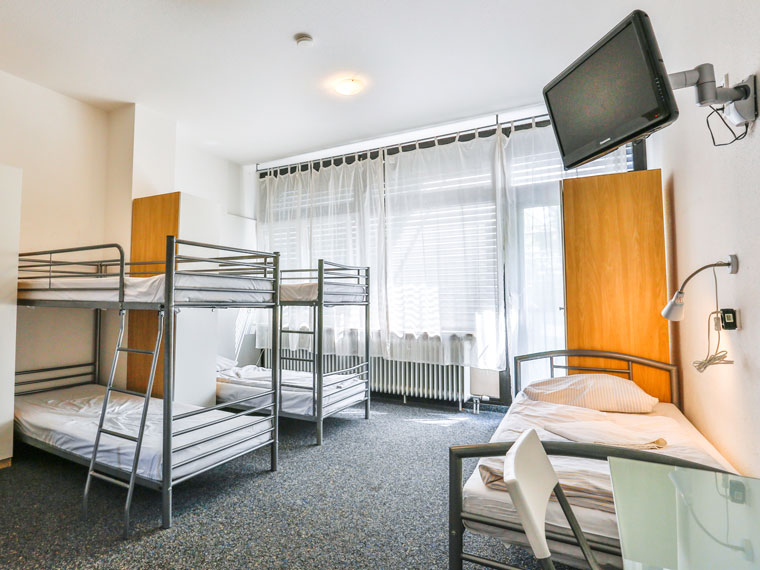
\includegraphics[width=0.5\linewidth]{images/accommodation/kaiserpassage/mehrbettzimmer-2.jpg}%
    };
    \node[inner sep=0,outer sep=0,anchor=north west] (sub-1) at (main.north east) {%
      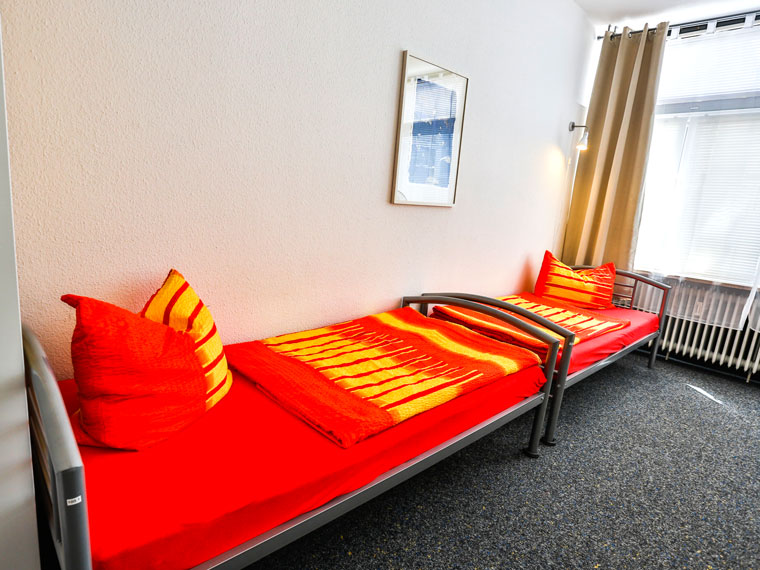
\includegraphics[width=0.25\linewidth]{images/accommodation/kaiserpassage/einzelzimmer.jpg}%
      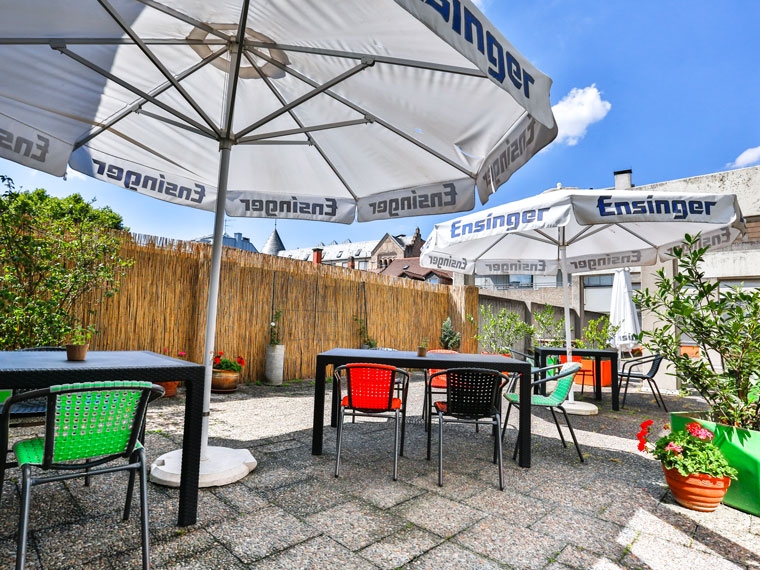
\includegraphics[width=0.25\linewidth]{images/accommodation/kaiserpassage/terasse.jpg}%
    };
    \node[inner sep=0,outer sep=0,anchor=north west] (sub-2) at (sub-1.south west) {%
      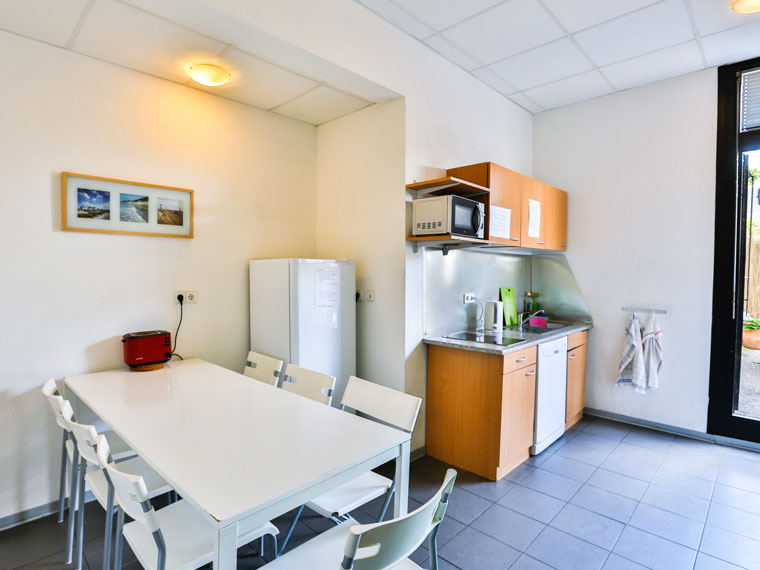
\includegraphics[width=0.25\linewidth]{images/accommodation/kaiserpassage/gemeinschaftskueche.jpg}%
      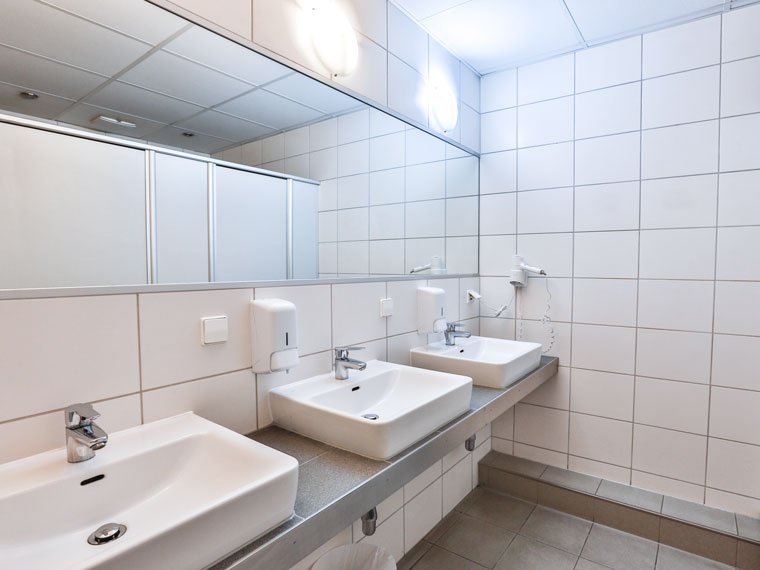
\includegraphics[width=0.25\linewidth]{images/accommodation/kaiserpassage/badezimmer.jpg}%
    };
  \end{scope}
  \node[anchor=south west,color=black,xshift=1ex,yshift=1ex] (label) at (main.south west) {\imgtitle{gloveler GmbH}{Gästehaus Kaiserpassage}{non-free, permission to use for bid}};
  \begin{scope}[on background layer]
    \node[fit=(label),inner sep=0,outer sep=0,opacity=0.6,fill=white,rounded corners] {};
  \end{scope}
\end{tikzpicture}

\begin{labeling}{\bf Availability}
  \item[\bf Location] West of City Center
  \item[\bf Price] \num{20} to \SI{22}{\euro/{pP}} in 4 bed room
  \item[\bf Breakfast] not available
  \item[\bf Availability] available
\end{labeling}

This small hostel is located in the western part of the city center. The hostel
does not offer breakfast or en-suite bathrooms. The hostel offers a shared
kitchen.

\subsection{B\&B Hotels}

\begin{labeling}{\bf Availability}
  \item[\bf Location] Main Station
  \item[\bf Price] \SI{33}{\euro/{pP}} in 2 bed room, \SI{28.70}{\euro/{pP}} in 3 bed room
  \item[\bf Breakfast] \SI{7,50}{\euro/{pP}}
  \item[\bf Availability] available
\end{labeling}

This is a relatively cheap hotel just behind the main station.


\newpage
